% Compiling: Use Overleaf with PDFLaTeX or `latexmk -pdf martian_habitability_proposal.tex`.
% Uses example-image to compile without external files.
% All TikZ graphics (bar chart, subsurface schematic, phase diagram) are self-contained.

\documentclass{beamer}
\usetheme{Madrid}
\usecolortheme{whale}
\usepackage[utf8]{inputenc}
\usepackage[T1]{fontenc}
\usepackage{lmodern}
\usepackage{amsmath,amsfonts,amssymb}
\usepackage{graphicx}
\usepackage{xcolor}
\usepackage{booktabs}
\usepackage{tikz}
\usetikzlibrary{patterns,arrows.meta,positioning}
\usepackage{pgfplots} % Added for axis environment
\pgfplotsset{compat=1.18} % Set PGFPlots compatibility
\usepackage{hyperref}
\usepackage{mwe} % For example-image
\usepackage{noto} % Font package, loaded last

% Custom colors
\definecolor{deepred}{RGB}{139,0,0}
\definecolor{deepblue}{RGB}{0,51,102}
\setbeamercolor{title}{fg=deepblue}
\setbeamercolor{frametitle}{fg=deepred}
\setbeamercolor{block title}{fg=deepblue,bg=gray!10}
\setbeamercolor{block body}{bg=gray!5}

% Title information
\title{\textbf{Zona de Habitabilidad Subsuperficial en Marte}}
\subtitle{Condiciones para Agua Líquida y Potencial Astrobiológico}
\author{[Tu Nombre]}
\institute{[Tu Institución]}
\date{\today}

\begin{document}

% Title slide
\begin{frame}
  \titlepage
  \begin{center}
    \includegraphics[width=0.3\textwidth]{example-image}
  \end{center}
\end{frame}

% Outline slide
\begin{frame}{Contenido}
  \tableofcontents
\end{frame}

% Introduction section
\section{Introducción}
\begin{frame}{Introducción}
  \begin{block}{Contexto}
    La superficie marciana ($T \sim -60^{\circ}\mathrm{C}$, $P \sim 6-8$ mbar) es inhóspita, pero el subsuelo ofrece:
    \begin{itemize}
      \item Gradiente geotérmico ($\sim 6-10$ K/km).
      \item Presión litostática creciente.
      \item Sales que reducen el punto de congelación.
    \end{itemize}
  \end{block}
  \begin{block}{Relevancia}
    Identificar zonas habitables subsuperficiales guía la búsqueda de vida en Marte.
  \end{block}
\end{frame}

% Objectives section
\section{Objetivos}
\begin{frame}{Objetivos}
  \begin{block}{Objetivo General}
    Caracterizar las condiciones del subsuelo marciano para agua líquida y su potencial astrobiológico.
  \end{block}
  \begin{block}{Objetivos Específicos}
    \begin{enumerate}
      \item Estimar profundidades para agua pura y salina.
      \item Analizar el efecto de sales (percloratos, cloruros).
      \item Evaluar la habitabilidad de salmueras.
    \end{enumerate}
  \end{block}
\end{frame}

% Methodology section
\section{Metodología}
\begin{frame}{Metodología}
  \begin{columns}
    \column{0.5\textwidth}
      \begin{itemize}
        \item \textbf{Diseño:} Modelado termodinámico y geofísico.
        \item \textbf{Datos:} Misiones Phoenix, Curiosity, InSight, Mars Express.
        \item \textbf{Técnicas:}
          \begin{itemize}
            \item Simulaciones de gradientes geotérmicos.
            \item Análisis de radar (MARSIS) y sismología.
          \end{itemize}
      \end{itemize}
    \column{0.5\textwidth}
      \begin{figure}
        \centering
        \includegraphics[width=0.8\textwidth]{example-image}
        \caption{Perfil de radar MARSIS a $\sim 1.5$ km bajo el polo sur. \cite{orosei2018}}
      \end{figure}
  \end{columns}
\end{frame}

% Preliminary Results section
\section{Resultados Preliminares}
\begin{frame}{Resultados Preliminares}
  \begin{block}{Profundidades Estimadas}
    Modelos sugieren:
    \begin{itemize}
      \item Agua pura: $\sim 8$ km (ecuador).
      \item Salmueras: $\sim 3-6$ km (latitudes bajas-medias).
    \end{itemize}
  \end{block}
  \begin{figure}
    \centering
    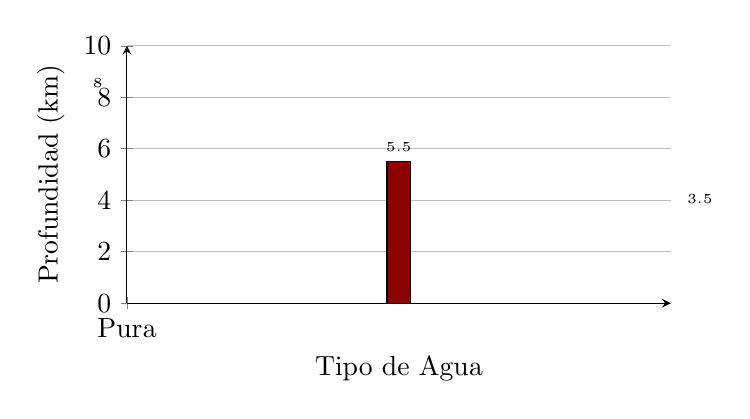
\begin{tikzpicture}
      \begin{axis}[
        ybar,
        bar width=0.3cm,
        width=0.7\textwidth,
        height=0.4\textwidth,
        ymin=0, ymax=10,
        ylabel={Profundidad (km)},
        xlabel={Tipo de Agua},
        xtick=data,
        xticklabels={Pura, Salina Moderada, Eutéctica},
        axis lines=left,
        grid=major,
        nodes near coords,
        every node near coord/.append style={font=\tiny}
      ]
      \addplot[fill=deepblue] coordinates {(1,8)};
      \addplot[fill=deepred] coordinates {(2,5.5)};
      \addplot[fill=gray] coordinates {(3,3.5)};
      \end{axis}
    \end{tikzpicture}
    \caption{Profundidades para agua líquida en el ecuador.}
  \end{figure}
\end{frame}

% Subsurface Structure section
\section{Estructura Subsuperficial}
\begin{frame}{Estructura Subsuperficial}
  \begin{figure}
    \centering
    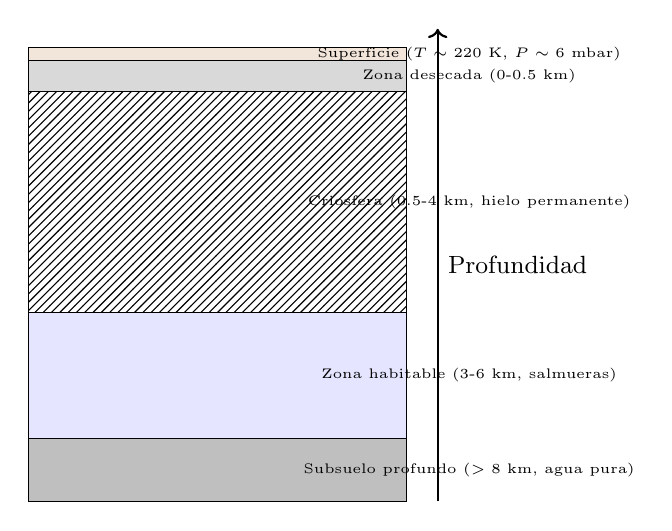
\begin{tikzpicture}[
      scale=0.8,
      layer/.style={rectangle, draw, fill=#1, minimum height=0.5cm, minimum width=6cm},
      annotation/.style={font=\tiny, align=left}
    ]
      % Surface
      \draw[fill=brown!20] (0,0) rectangle (6,0.2);
      \node[annotation] at (7,0.1) {Superficie ($T \sim 220$ K, $P \sim 6$ mbar)};
      % Desiccated zone
      \draw[fill=gray!30] (0,-0.5) rectangle (6,0);
      \node[annotation] at (7,-0.25) {Zona desecada (0-0.5 km)};
      % Cryosphere
      \draw[fill=cyan!20, pattern=north east lines] (0,-4) rectangle (6,-0.5);
      \node[annotation] at (7,-2.25) {Criosfera (0.5-4 km, hielo permanente)};
      % Habitable zone
      \draw[fill=blue!10] (0,-6) rectangle (6,-4);
      \node[annotation] at (7,-5) {Zona habitable (3-6 km, salmueras)};
      % Deep subsurface
      \draw[fill=gray!50] (0,-7) rectangle (6,-6);
      \node[annotation] at (7,-6.5) {Subsuelo profundo ($>8$ km, agua pura)};
      % Arrows
      \draw[->, thick] (6.5,-7) -- (6.5,0.5) node[midway, right, font=\small] {Profundidad};
    \end{tikzpicture}
    \caption{Esquema de la estructura subsuperficial marciana.}
  \end{figure}
\end{frame}

% Phase Diagram section
\section{Diagrama de Fases}
\begin{frame}{Diagrama de Fases}
  \begin{figure}
    \centering
    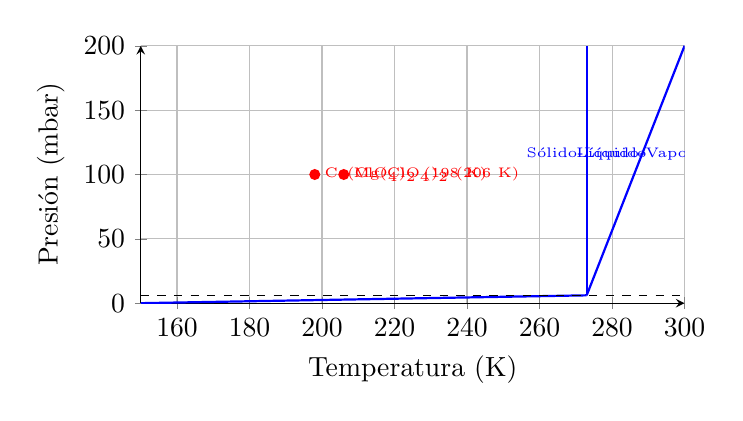
\begin{tikzpicture}
      \begin{axis}[
        width=0.7\textwidth,
        height=0.4\textwidth,
        xlabel={Temperatura (K)},
        ylabel={Presión (mbar)},
        xmin=150, xmax=300,
        ymin=0, ymax=200, % Reduced ymax to prevent dimension errors
        grid=major,
        axis lines=left
      ]
      % Triple point of water
      \draw[thick, blue] (273,6.1) -- (273,200) node[midway, above, font=\tiny] {Sólido-Líquido};
      \draw[thick, blue] (273,6.1) -- (300,200) node[midway, above, font=\tiny] {Líquido-Vapor};
      \draw[thick, blue] (150,0) -- (273,6.1) node[midway, below, font=\tiny] {Sólido-Vapor};
      % Eutectic points
      \fill[red] (198,100) circle (2pt) node[right, font=\tiny] {Ca(ClO$_4$)$_2$ (198 K)};
      \fill[red] (206,100) circle (2pt) node[right, font=\tiny] {Mg(ClO$_4$)$_2$ (206 K)};
      % Mars surface pressure
      \draw[dashed] (150,6) -- (300,6) node[right, font=\tiny] {P superficial $\sim 6$ mbar};
      \end{axis}
    \end{tikzpicture}
    \caption{Diagrama de fases simplificado con puntos eutécticos de salmueras.}
  \end{figure}
\end{frame}

% Expected Results section
\section{Resultados Esperados}
\begin{frame}{Resultados Esperados}
  \begin{itemize}
    \item Mapa de profundidades habitables (3-8 km).
    \item Confirmación del rol de percloratos en salmueras.
    \item Priorización de sitios para exploración.
  \end{itemize}
  \begin{block}{Impacto}
    Guía para misiones como ExoMars y Perseverance.
  \end{block}
\end{frame}

% Astrobiological Implications section
\section{Implicaciones}
\begin{frame}{Implicaciones Astrobiológicas}
  \begin{itemize}
    \item \textbf{Hábitats:} Salmueras a $>3$ km para microbios quimiolitótrofos.
    \item \textbf{Energía:} Radiólisis, serpentinización.
    \item \textbf{Límites:} Salinidad ($a_w \sim 0.5$) y frío extremo.
  \end{itemize}
\end{frame}

% Timeline section
\section{Cronograma}
\begin{frame}{Cronograma}
  \begin{table}
    \centering
    \begin{tabular}{l|c|c|c|c}
      \toprule
      \textbf{Actividad} & \textbf{Mes 1-3} & \textbf{4-6} & \textbf{7-9} & \textbf{10-12} \\
      \midrule
      Revisión bibliográfica & \checkmark & & & \\
      Recolección de datos & \checkmark & \checkmark & & \\
      Modelado & & \checkmark & \checkmark & \\
      Análisis astrobiológico & & & \checkmark & \checkmark \\
      Redacción & & & & \checkmark \\
      \bottomrule
    \end{tabular}
    \caption{Cronograma del proyecto.}
  \end{table}
\end{frame}

% References section
\section{Referencias}
\begin{frame}{Referencias}
  \begin{thebibliography}{10}
    \bibitem{orosei2018} Orosei et al. (2018). \emph{Radar evidence of subglacial liquid water.} Science, 361:490-493.
    \bibitem{chevrier2009} Chevrier et al. (2009). \emph{Stability of perchlorate hydrates.} Geophys. Res. Lett., 36:L10202.
    \bibitem{tarnas2021} Tarnas et al. (2021). \emph{Earth-like habitable environments.} Astrobiology, 21:741-756.
  \end{thebibliography}
\end{frame}

% Final slide
\begin{frame}{Gracias}
  \centering
  \Huge{\textbf{¡Gracias por su atención!}}
  \vfill
  \normalsize{Contacto: \href{mailto:tu.correo@dominio.com}{tu.correo@dominio.com}}
\end{frame}

\end{document}